%!TEX root = slides.tex
%!TEX program = xelatex
% (für das LaTeXtools Sublime plugin)

\documentclass{beamer}

%Blablabla front matter....

\title{Quantum Key Distribution}
\subtitle{Foundational Aspects of Quantum Mechanics}
\date{01-02-2017}
\author[Hirscher, Snijders]{Simon Hirscher \& Max Snijders}

%\setbeameroption{show notes}
%\setbeamertemplate{note page}[plain]

\usepackage[LastSlideNotCounted,ProgressBar,NoPageCounter]{beamer-template-mk-i/beamerthememxmki}
\hypersetup{pdfpagemode=FullScreen}

% Use this for the handout!

% \usepackage{pgfpages}
% \pgfpagesuselayout{4 on 1}[a4paper]

% Quotes are awesome! (Sometimes)

\newcommand*{\openquote}{\tikz[remember picture,overlay,xshift=-15pt,yshift=-10pt]
	\node (OQ) {\fontsize{60}{60}\selectfont``};\kern0pt}
\newcommand*{\closequote}{\tikz[remember picture,overlay,xshift=15pt,yshift=10pt]
	\node (CQ) {\fontsize{60}{60}\selectfont''};}
% select a colour for the shading
\definecolor{shadecolor}{named}{white}
% wrap everything in its own environment
\newenvironment{shadequote}%
{\begin{quote}\openquote}
		{\hfill\closequote\end{quote}}


% And now for the real deal...
\begin{document}
	\section{Introduction} % Simon
	\begin{frame}
		\begin{center}
		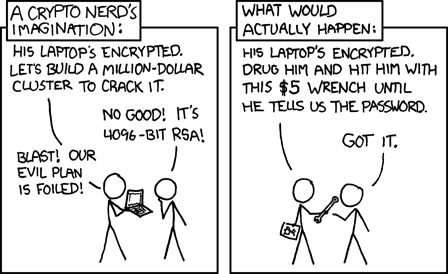
\includegraphics[width=0.8\textwidth]{images/xkcd-security.png}
		\end{center}
	\end{frame}

	\begin{frame}
		\titlepage
	\end{frame}

	% Structure of the talk
	\begin{frame}{Contents} % Simon

	\end{frame}

	% Opener: Why do we need encryption?
	\begin{frame}{Encryption} % Simon

	\end{frame}

	% Elementary encryption techniques.
	\section{Encryption Techniques}

	\begin{frame}{Shifting Caesar Cipher} % Max
		\note{Anything typed here will be outputted with the handouts}
	\end{frame}

	\begin{frame}{Permutative Caesar Cipher} % Max

	\end{frame}

	\begin{frame}{XOR} % Simon

	\end{frame}

	\begin{frame}{One-Time Pad} % Simon

	\end{frame}

	% Key distribution section
	\section{Key Distribution}

	\begin{frame}{Diffie-Hellman} % Max

	\end{frame}

	\begin{frame}{Public/Private Key} % Simon

	\end{frame}

	\begin{frame}{Quantum Key Exchange} % Max

	\end{frame}

	% Methods of Quantum Key Exchange
	\section{Quantum Key Exchange}

	\begin{frame}{BB-84} % Max

	\end{frame}

	\begin{frame}{E-91} % Simon

	\end{frame}

	% Authentication Requirement
	\section{Authentication}

	\begin{frame}{Public/Private Key Authentication} % Simon

	\end{frame}

	% Hacks
	\section{Vulnerabilities}

	\begin{frame}{Sender basis detection} % Max

	\end{frame}


	% A black slide to end the talk
	\setbeamercolor{background canvas}{bg=black}
	\begin{frame}[plain]\end{frame}

\end{document}